\section{Implementation Results}
\label{sec:results}
\subsection{Completed Runs and Evidence Coverage}
The evidence contains five models at seeds 69420, 67 and 69: 15 main runs and
30 best/last checkpoints. All runs record clean source revision \texttt{a8539be},
protocol \texttt{a1-v0}, the same seed-36 split and the same normalization identity.
Eleven runs reached 100 epochs. Linear completed 38/33/31 epochs and MLP seed 67
completed 83, consistent with their configured stopping policy. Full IDs and
per-seed results are in Appendix~\ref{app:runs}.

The training notebook originally produced validation-only results. A separate
postprocessing stage restored every selected checkpoint, replayed validation and
then evaluated the official test partition. Its 30 evaluations each contain
10,000 predictions, totaling 300,000 saved rows. These are repeated evaluations
of the same validation/test images, not 300,000 independent samples.

Artifact checks verified 61 completion markers, source/config/checkpoint identities,
prediction IDs, class support, confusion matrices, per-class scores and seed
aggregates. Accuracy/F1 replay matches training validation exactly; the largest
loss change is \(3.84\times10^{-8}\). Lack of GPU availability in that evaluation
session caused its GPU timing stage to be skipped, not its test evaluation.
The separately retained Windows CPU timing profile supplies the inference
measurements reported below. No additional training was needed for these stages.

\subsection{Main Quantitative Comparison}
Table~\ref{tab:performance} reports selected-checkpoint validation and official-test
metrics, using all three seeds without selecting a test winner.
Validation supports model selection and is not an independent final assessment.
\begin{table}[H]\centering\small
\caption{Mean \(\pm\) sample SD over three seeds. Accuracy/F1 are percentages;
CE is sample-weighted cross-entropy.}
\label{tab:performance}
\begin{tabular}{llrrr}
\toprule
Model & Split & Accuracy (\%) & Macro-F1 (\%) & CE loss \\
\midrule
Linear & Val. & 79.267 $\pm$ 0.176 & 79.254 $\pm$ 0.159 & 0.58673 $\pm$ 0.00234 \\
Linear & Test & 78.377 $\pm$ 0.283 & 78.427 $\pm$ 0.307 & 0.61142 $\pm$ 0.00292 \\
MLP & Val. & 90.333 $\pm$ 0.165 & 90.288 $\pm$ 0.157 & 0.26488 $\pm$ 0.00057 \\
MLP & Test & 89.720 $\pm$ 0.104 & 89.698 $\pm$ 0.094 & 0.28806 $\pm$ 0.00258 \\
CNN & Val. & 91.547 $\pm$ 0.115 & 91.556 $\pm$ 0.056 & 0.24148 $\pm$ 0.00427 \\
CNN & Test & 90.690 $\pm$ 0.324 & 90.726 $\pm$ 0.262 & 0.26421 $\pm$ 0.00855 \\
GRU & Val. & 91.063 $\pm$ 0.061 & 91.055 $\pm$ 0.064 & 0.26549 $\pm$ 0.00438 \\
GRU & Test & 90.297 $\pm$ 0.255 & 90.281 $\pm$ 0.250 & 0.28357 $\pm$ 0.00235 \\
Transformer & Val. & 91.580 $\pm$ 0.026 & 91.548 $\pm$ 0.011 & 0.23699 $\pm$ 0.00250 \\
Transformer & Test & 91.267 $\pm$ 0.237 & 91.234 $\pm$ 0.215 & 0.24440 $\pm$ 0.00402 \\
\bottomrule
\end{tabular}

\end{table}

The Transformer has the highest mean test accuracy (91.267\%) and macro-F1
(91.234\%), compared with 90.690\% and 90.726\% for CNN. The differences are
0.577 and 0.508 percentage points. Paired Transformer--CNN test-accuracy
differences are \(+0.81,+0.62,+0.30\) points at seeds 69420, 67 and 69.
This is consistent across the three observed seeds, but does not establish
statistical significance or superiority on other datasets.

The MLP improves substantially over Linear (89.720\% versus 78.377\% test accuracy),
and GRU reaches 90.297\%. Across these runs, test-accuracy sample SD ranges from
0.104 to 0.324 percentage points. The small number of seeds limits inference about
the wider run distribution. Figure~\ref{fig:comparison} visualizes the same test
means and SDs.
\begin{figure}[H]\centering
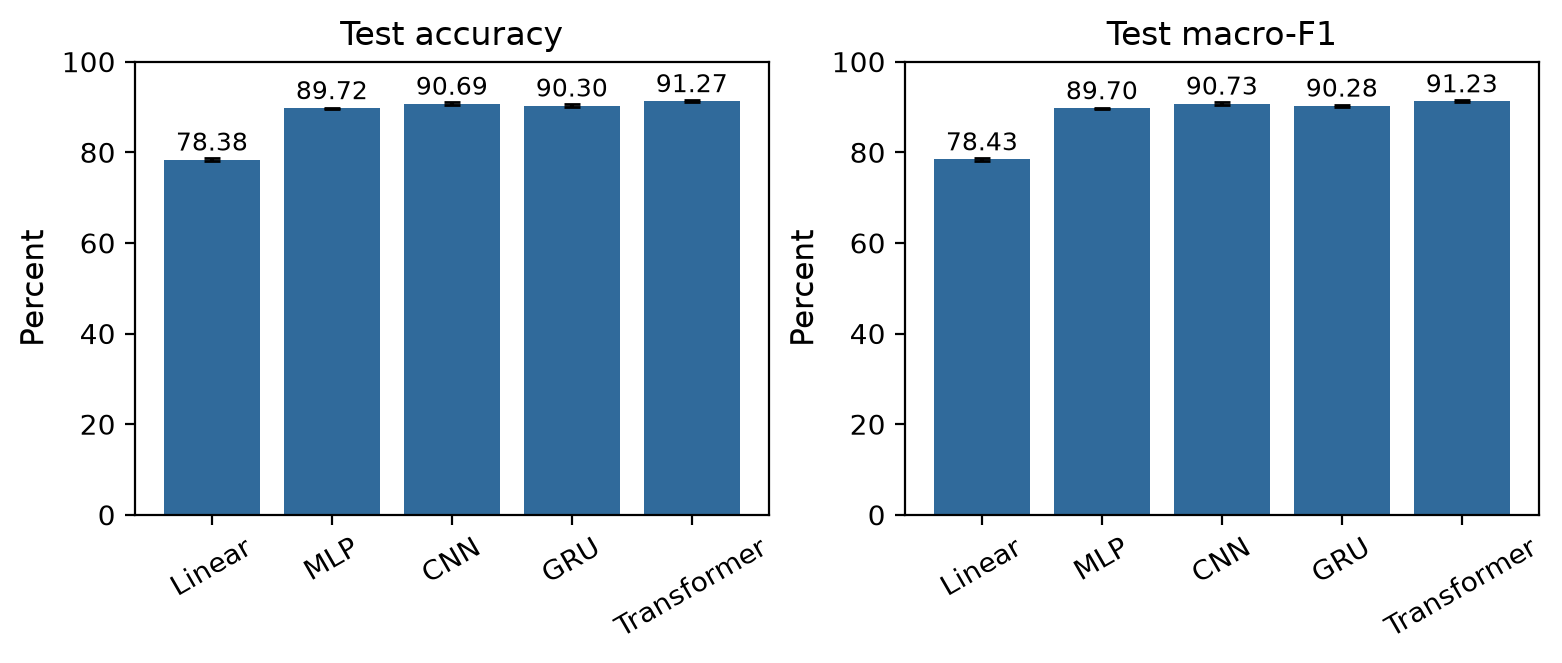
\includegraphics[width=\linewidth]{figures/comparison.png}
\caption{Official-test accuracy and macro-F1: mean with sample-SD error bars,
\(n=3\). Both axes retain the 0--100 percent scale.}
\label{fig:comparison}
\end{figure}

Table~\ref{tab:parameters} separates total, trainable and frozen parameter elements.
All five recorded architectures are fully trainable. Buffers are not parameters.
CNN uses about 72.9\% fewer parameters than Transformer while remaining close
in predictive quality; the larger MLP does not obtain the strongest scores.
\begin{table}[H]\centering\small
\caption{Exact parameter counts of the reported configurations.}
\label{tab:parameters}
\begin{tabular}{lrrr}
\toprule
Model & Total & Trainable & Frozen \\
\midrule
Linear & 7,850 & 7,850 & 0 \\
MLP & 235,146 & 235,146 & 0 \\
CNN & 28,426 & 28,426 & 0 \\
GRU & 61,962 & 61,962 & 0 \\
Transformer & 104,970 & 104,970 & 0 \\
\bottomrule
\end{tabular}

\end{table}
\FloatBarrier

\subsection{Learning Dynamics and Convergence}
Figures~\ref{fig:learn-linear}--\ref{fig:learn-transformer} show seed 67 for each
model. The vertical line marks the saved best-validation checkpoint, using
1-based epochs. The selected epoch need not be the final epoch.

\begin{figure}[H]\centering
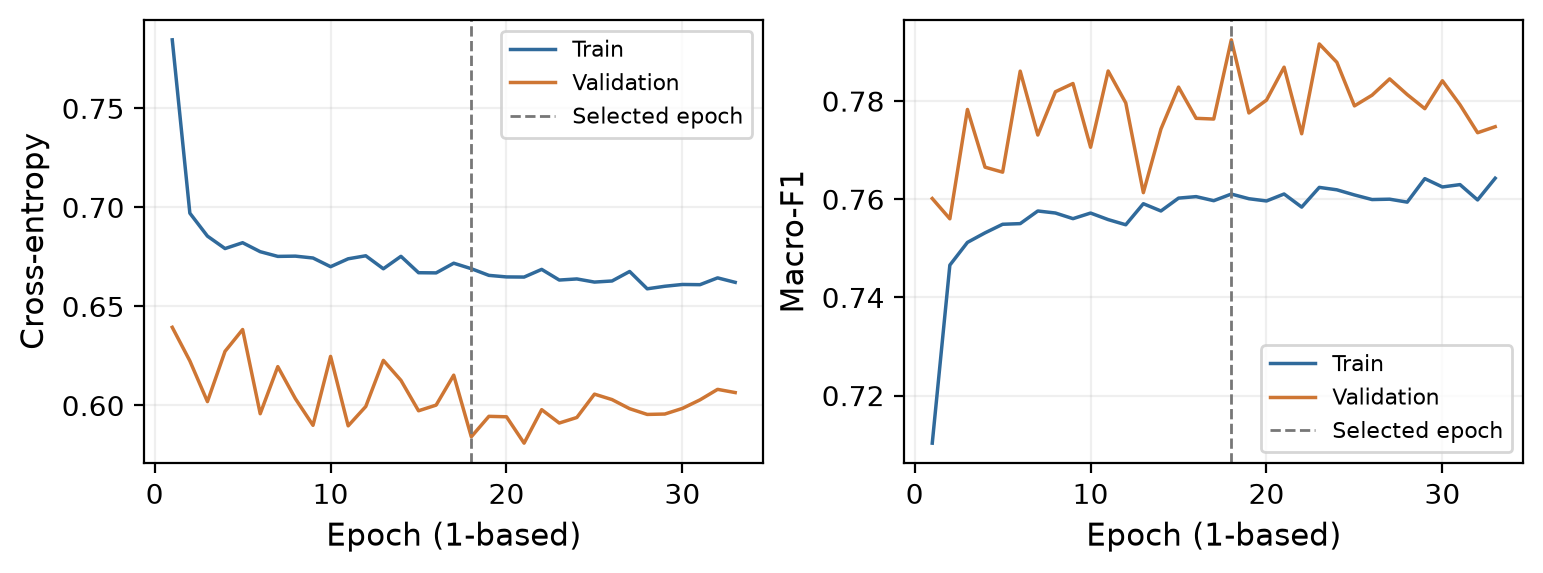
\includegraphics[width=\linewidth]{figures/learning_linear.png}
\caption{Linear learning history, seed 67: training/validation loss and macro-F1.}
\label{fig:learn-linear}
\end{figure}

\begin{figure}[H]\centering
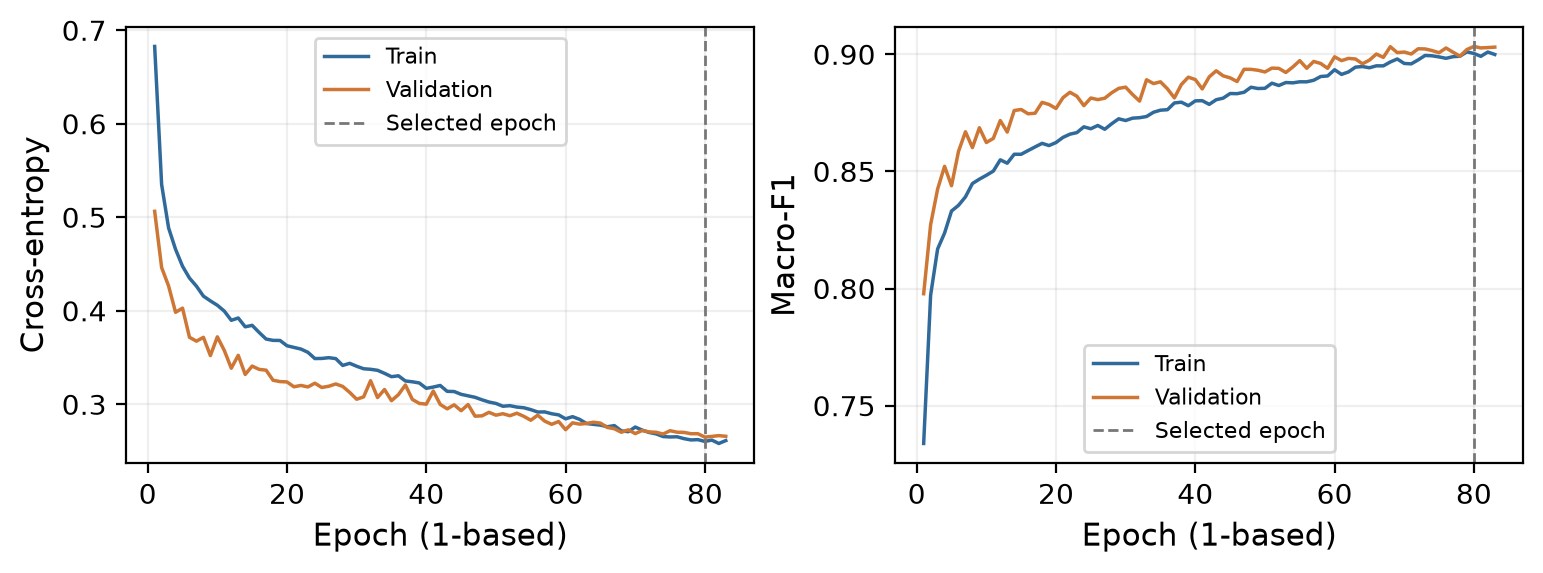
\includegraphics[width=\linewidth]{figures/learning_mlp.png}
\caption{MLP learning history, seed 67: training/validation loss and macro-F1.}
\label{fig:learn-mlp}
\end{figure}

\begin{figure}[H]\centering
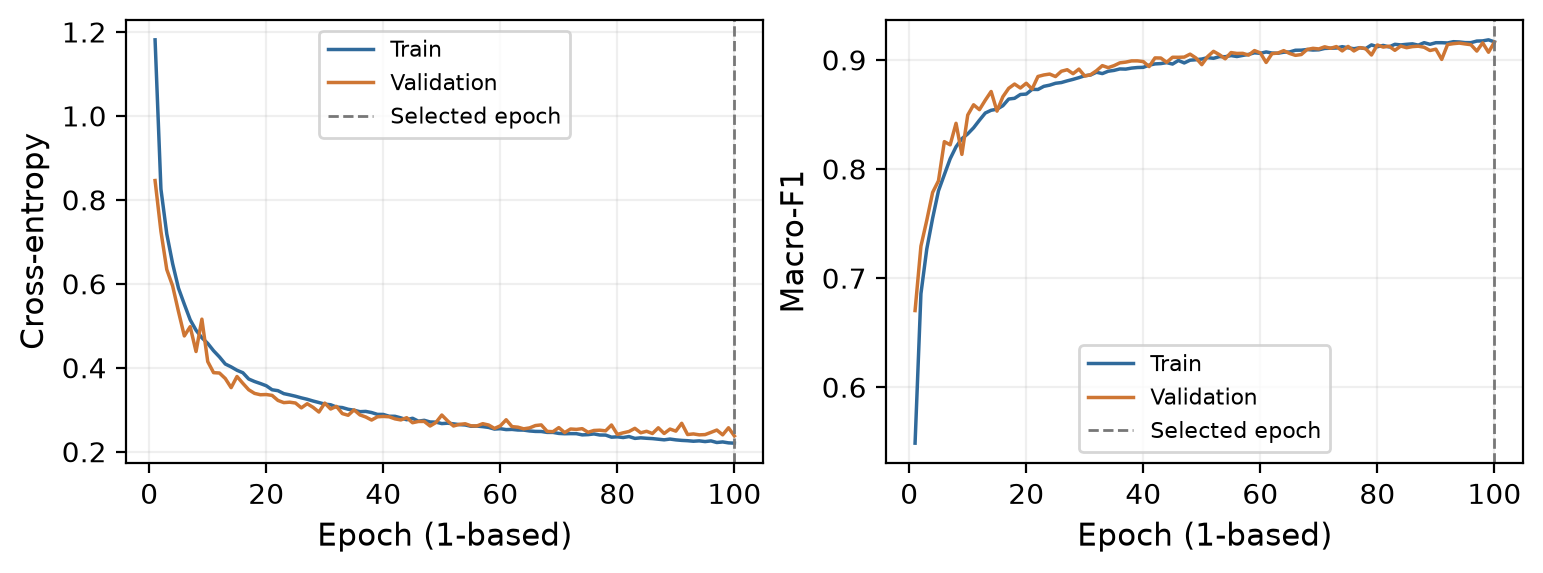
\includegraphics[width=\linewidth]{figures/learning_cnn.png}
\caption{CNN learning history, seed 67: training/validation loss and macro-F1.}
\label{fig:learn-cnn}
\end{figure}

\begin{figure}[H]\centering
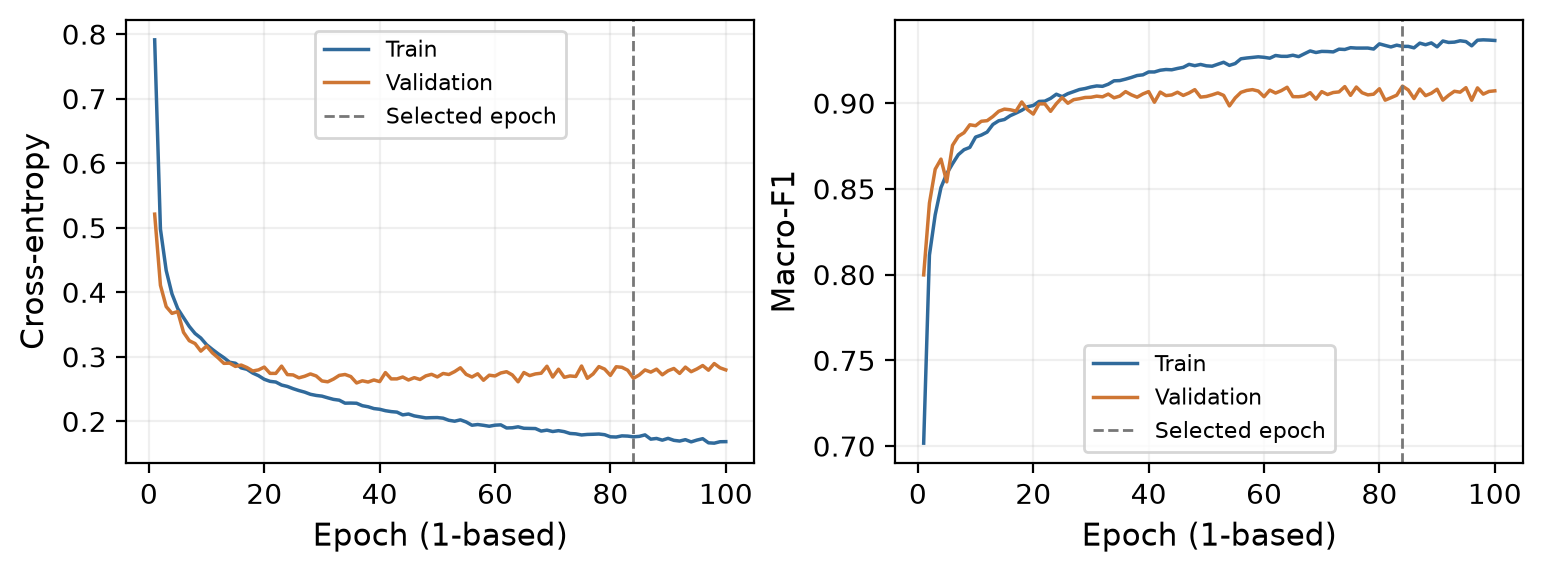
\includegraphics[width=\linewidth]{figures/learning_rnn.png}
\caption{GRU learning history, seed 67: training/validation loss and macro-F1.}
\label{fig:learn-rnn}
\end{figure}

\begin{figure}[H]\centering
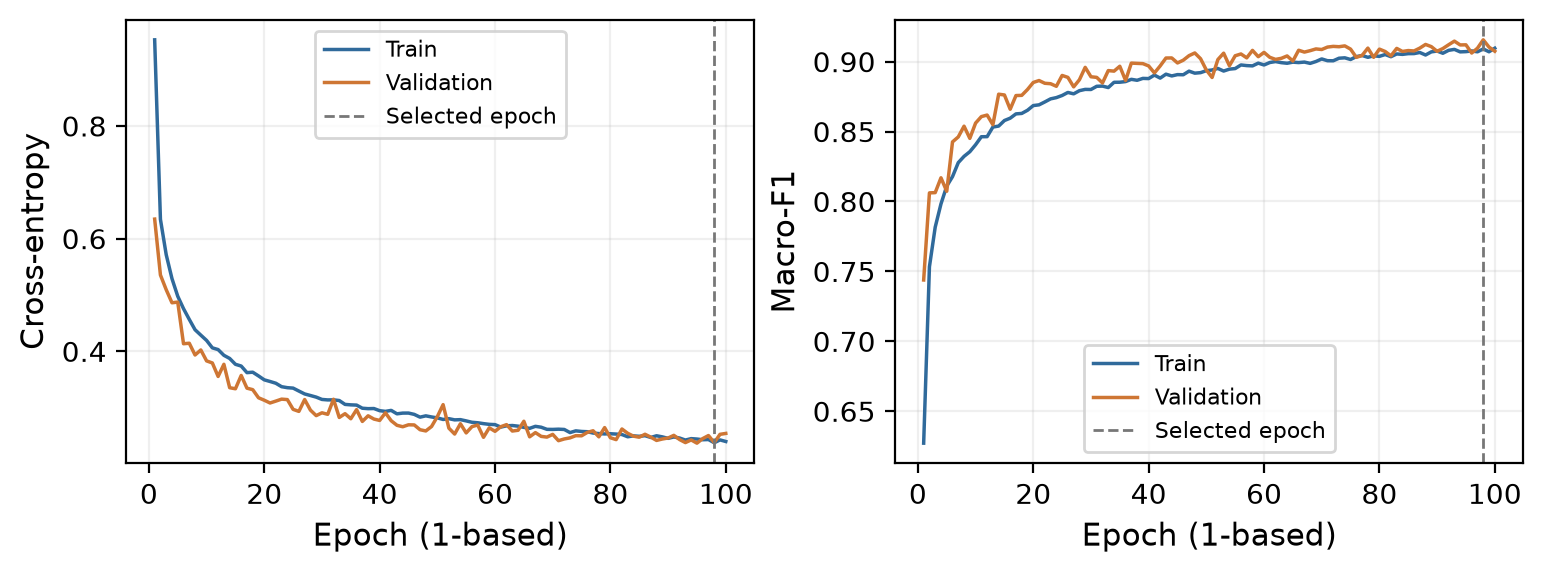
\includegraphics[width=\linewidth]{figures/learning_transformer.png}
\caption{Transformer learning history, seed 67: training/validation loss and macro-F1.}
\label{fig:learn-transformer}
\end{figure}

Linear stabilizes at much lower F1 and fluctuates after early improvement.
MLP, CNN and Transformer improve rapidly before making smaller late gains;
their observed training and validation curves remain relatively close.
These training curves include augmentation and dropout effects, while validation
uses deterministic preprocessing and evaluation mode.

GRU shows the clearest late divergence: training F1 continues improving while
validation F1 largely plateaus and validation loss rises slightly. Its seed-67
selected epoch is 84, before the final epoch 100. This pattern suggests that
continuing optimization does not keep improving held-out validation performance.
It does not prove a single causal mechanism. Best epochs for the other seed-67
runs are Linear 18, MLP 80, CNN 100 and Transformer 98.
\FloatBarrier

\subsection{Efficiency and Accuracy--Compute Trade-offs}
Table~\ref{tab:train-time} sums the saved \texttt{epoch\_seconds} values, each
of which surrounds training plus validation. It excludes full startup,
preparation and checkpoint overhead, and should not be read as isolated
forward/backward time.
\begin{table}[H]\centering\small
\caption{T4 train-and-validation epoch-loop cost. Epoch sequences and best
epochs are ordered by seeds 69420/67/69; times are mean \(\pm\) sample SD.}
\label{tab:train-time}
\begin{tabular}{lcr c}
\toprule
Model & Epochs & Loop time (min) & Best epochs \\
\midrule
Linear & 38 / 33 / 31 & 10.27 $\pm$ 1.05 & 30 / 18 / 16 \\
MLP & 100 / 83 / 100 & 29.85 $\pm$ 3.18 & 92 / 80 / 93 \\
CNN & 100 / 100 / 100 & 33.49 $\pm$ 0.44 & 100 / 100 / 81 \\
GRU & 100 / 100 / 100 & 32.89 $\pm$ 0.24 & 62 / 84 / 53 \\
Transformer & 100 / 100 / 100 & 38.39 $\pm$ 0.91 & 96 / 98 / 100 \\
\bottomrule
\end{tabular}

\end{table}
The Transformer has the largest observed loop cost (38.39 minutes), compared
with CNN's 33.49 minutes, a difference of about 4.90 minutes. Both use 100
epochs, but their per-epoch computation differs. Linear/MLP totals also reflect
their early-stopping policy and, for MLP, a shorter 83-epoch run. The MLP's
timing SD therefore includes a budget difference; it is not solely machine noise
or variation in model quality.

Table~\ref{tab:inference} reports the separate Windows CPU measurements under
Section~\ref{sec:environment}'s batch-64 forward-only protocol. A row averages
three per-checkpoint medians of 100 timed batches; SD describes those three
run-level values.
\begin{table}[H]\centering\small
\caption{Windows CPU forward-only timing: two threads, float32, batch 64,
20 warm-ups and 100 timed batches per checkpoint; \(n=3\).}
\label{tab:inference}
\begin{tabular}{lrrr}
\toprule
Model & Batch time (ms) & ms/image & Images/s \\
\midrule
Linear & 0.097 $\pm$ 0.003 & 0.001523 $\pm$ 0.000051 & 657237 $\pm$ 22106 \\
MLP & 1.151 $\pm$ 0.129 & 0.017987 $\pm$ 0.002016 & 56047 $\pm$ 6034 \\
CNN & 25.875 $\pm$ 2.663 & 0.404296 $\pm$ 0.041606 & 2491 $\pm$ 260 \\
GRU & 6.897 $\pm$ 2.059 & 0.107765 $\pm$ 0.032176 & 9776 $\pm$ 2494 \\
Transformer & 28.463 $\pm$ 3.584 & 0.444738 $\pm$ 0.056000 & 2273 $\pm$ 288 \\
\bottomrule
\end{tabular}

\end{table}
The Linear and MLP have much lower measured CPU cost than the other models.
CNN averages 0.404296 ms/image versus Transformer's 0.444738, so the Transformer
is about 10.0\% slower by these observed means. Their timing SDs are substantial,
and no formal claim of a stable speed ordering is made. GRU's mean is 0.107765
ms/image, giving a different quality--speed trade-off from its T4 training cost.
Throughput averages per-run rates; it need not equal the reciprocal of the rounded
aggregate latency.

These figures describe the documented CPU/library profile and preallocated input,
not end-to-end service performance. Parameter count alone does not predict runtime:
kernel structure, sequence processing and implementation matter, but their
individual contributions were not isolated. Deployment choices require measurements
on the intended hardware, batch size and input path.
\FloatBarrier

\subsection{Confusion Matrices and Class-Level Results}
\label{sec:confusion}
The following figures use the seed-67 official-test predictions; class metrics
quoted in the accompanying text refer to those same predictions.
They are representative single-run evidence; Table~\ref{tab:performance} remains
the three-seed comparison, and Appendix~\ref{app:class} reports aggregate class
metrics. Every figure uses the same raw-count color range, 0--1,000, and the same
class order.

There are 1,000 test examples per class. Consequently,
\(\mathrm{Recall}_c=C_{cc}/1000\); raw diagonal counts themselves are not recalls.
Because supports are equal, overall accuracy equals mean class recall.
Quoted precision, recall and F1 use the 0--1 scale. Full seed-level class metrics
are retained in the source CSV, and aggregate class tables appear in the appendix.

\clearpage
\subsubsection{Linear}
\begin{figure}[H]\centering
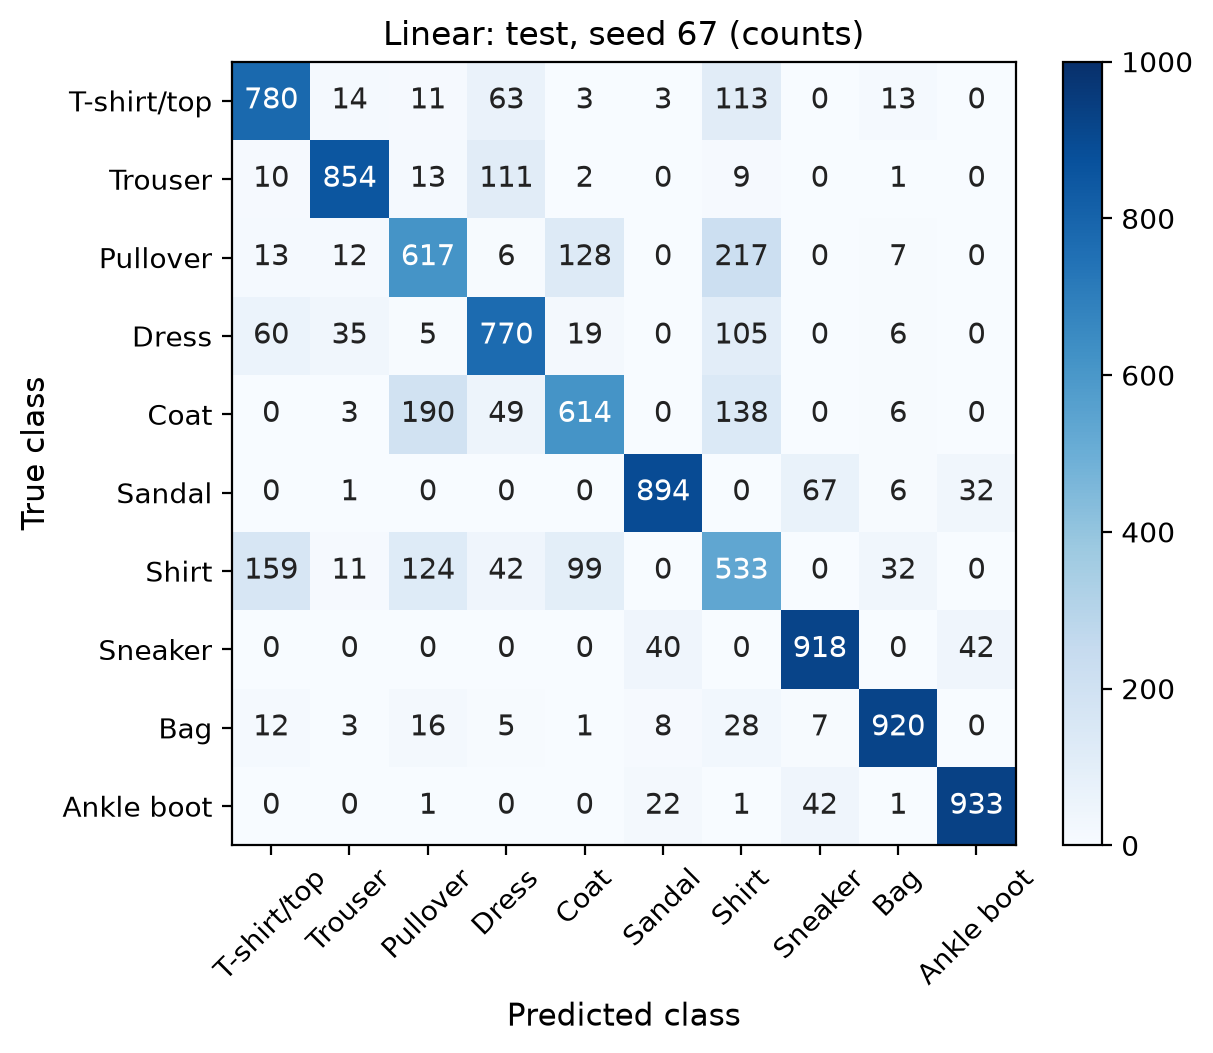
\includegraphics[width=.90\linewidth]{figures/confusion_linear.png}
\caption{Linear test confusion counts, seed 67; shared color scale 0--1,000.}
\label{fig:cm-linear}
\end{figure}
Linear's weakest class is Shirt (F1 0.497), with 159 Shirts predicted as
T-shirt/top, 124 as Pullover and 99 as Coat. Pullover/Coat confusion is also large:
128 Pullovers are predicted as Coat and 190 Coats as Pullover. This motivates
using nonlinear and spatial feature models, but the comparison does not isolate
representation from all other configuration differences.

\clearpage
\subsubsection{MLP}
\begin{figure}[H]\centering
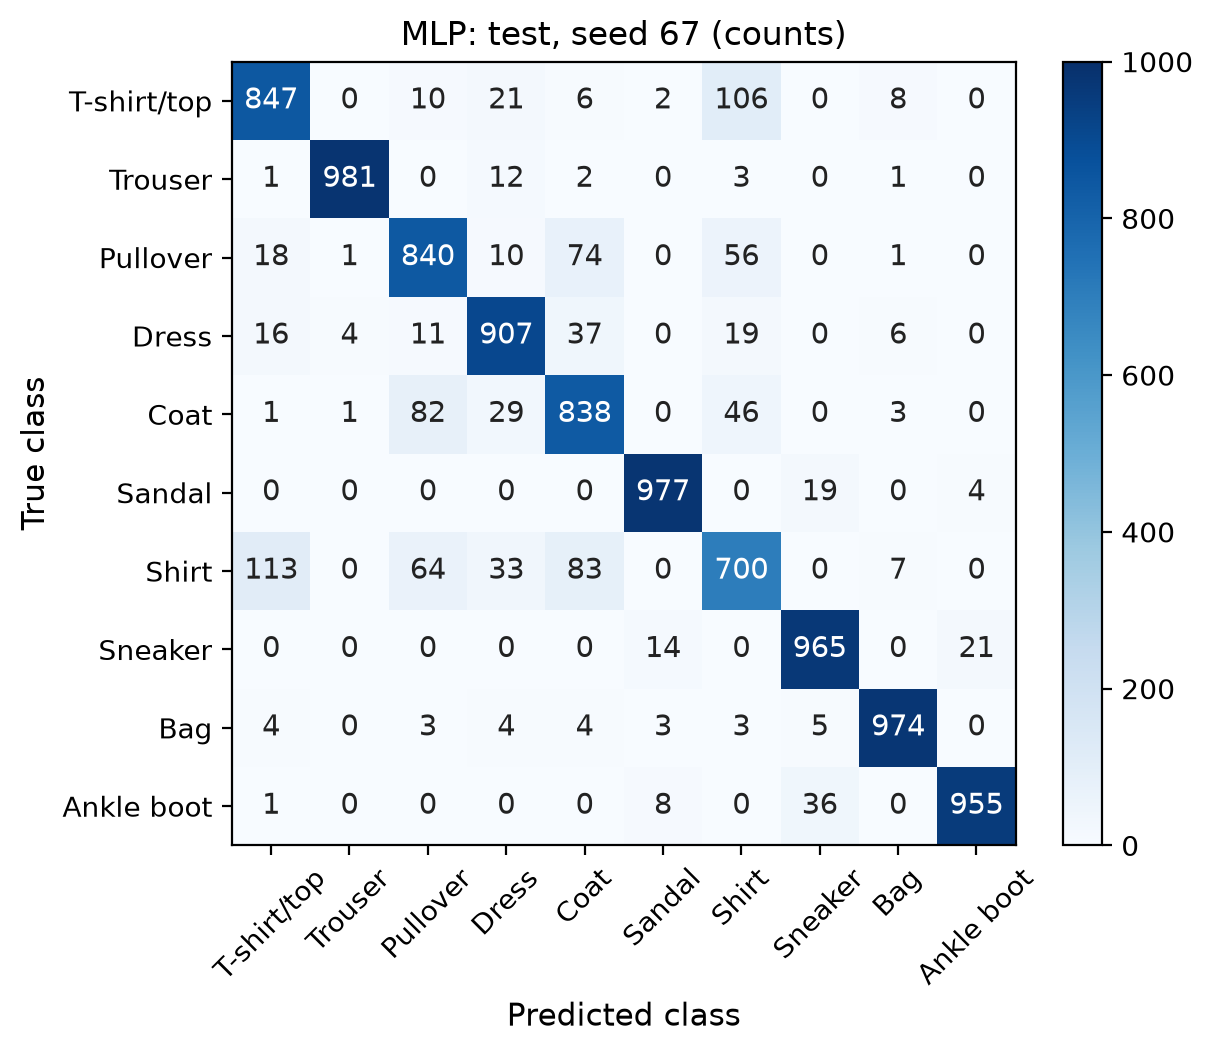
\includegraphics[width=.90\linewidth]{figures/confusion_mlp.png}
\caption{MLP test confusion counts, seed 67; shared color scale 0--1,000.}
\label{fig:cm-mlp}
\end{figure}
MLP improves overall accuracy to 89.84\% in this run. Trouser has F1 0.987,
while Shirt remains lowest at 0.724. There are 113 Shirt-to-T-shirt/top errors
and 106 in the reverse direction. Pullover--Coat errors persist (74 and 82 in
the two directions), showing that greater dense capacity does not eliminate
apparel ambiguity.

\clearpage
\subsubsection{CNN}
\begin{figure}[H]\centering
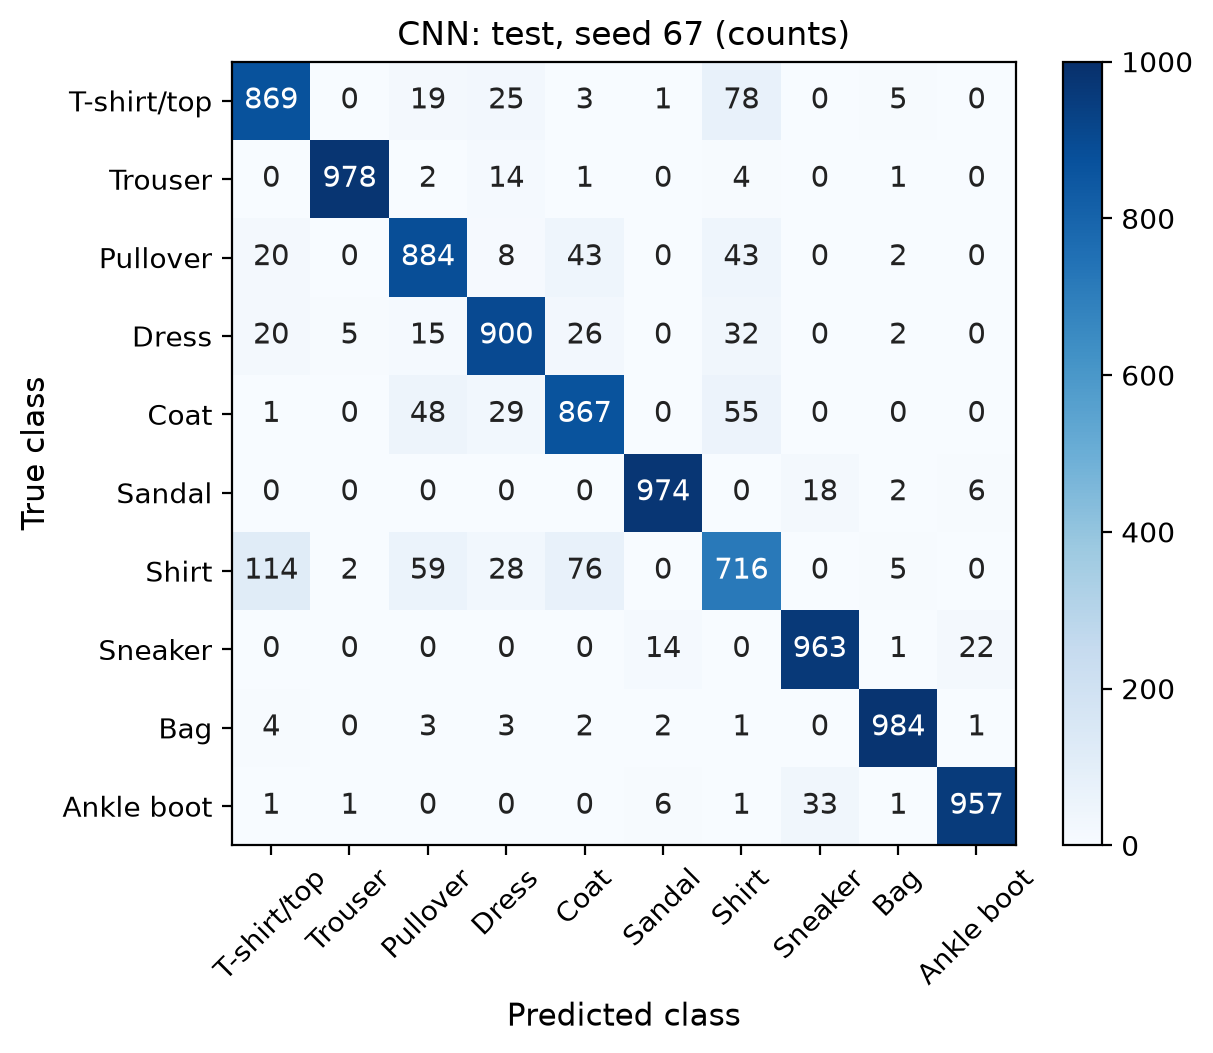
\includegraphics[width=.90\linewidth]{figures/confusion_cnn.png}
\caption{CNN test confusion counts, seed 67; shared color scale 0--1,000.}
\label{fig:cm-cnn}
\end{figure}
CNN reaches 90.92\% accuracy in this seed. Shirt remains weakest (F1 0.742);
114 Shirts are predicted as T-shirt/top, 76 as Coat and 59 as Pullover.
Pullover--Coat errors are lower than MLP's in both directions (43 and 48).
This is compatible with useful local image features, but is not a controlled
causal test of locality.

\clearpage
\subsubsection{GRU}
\begin{figure}[H]\centering
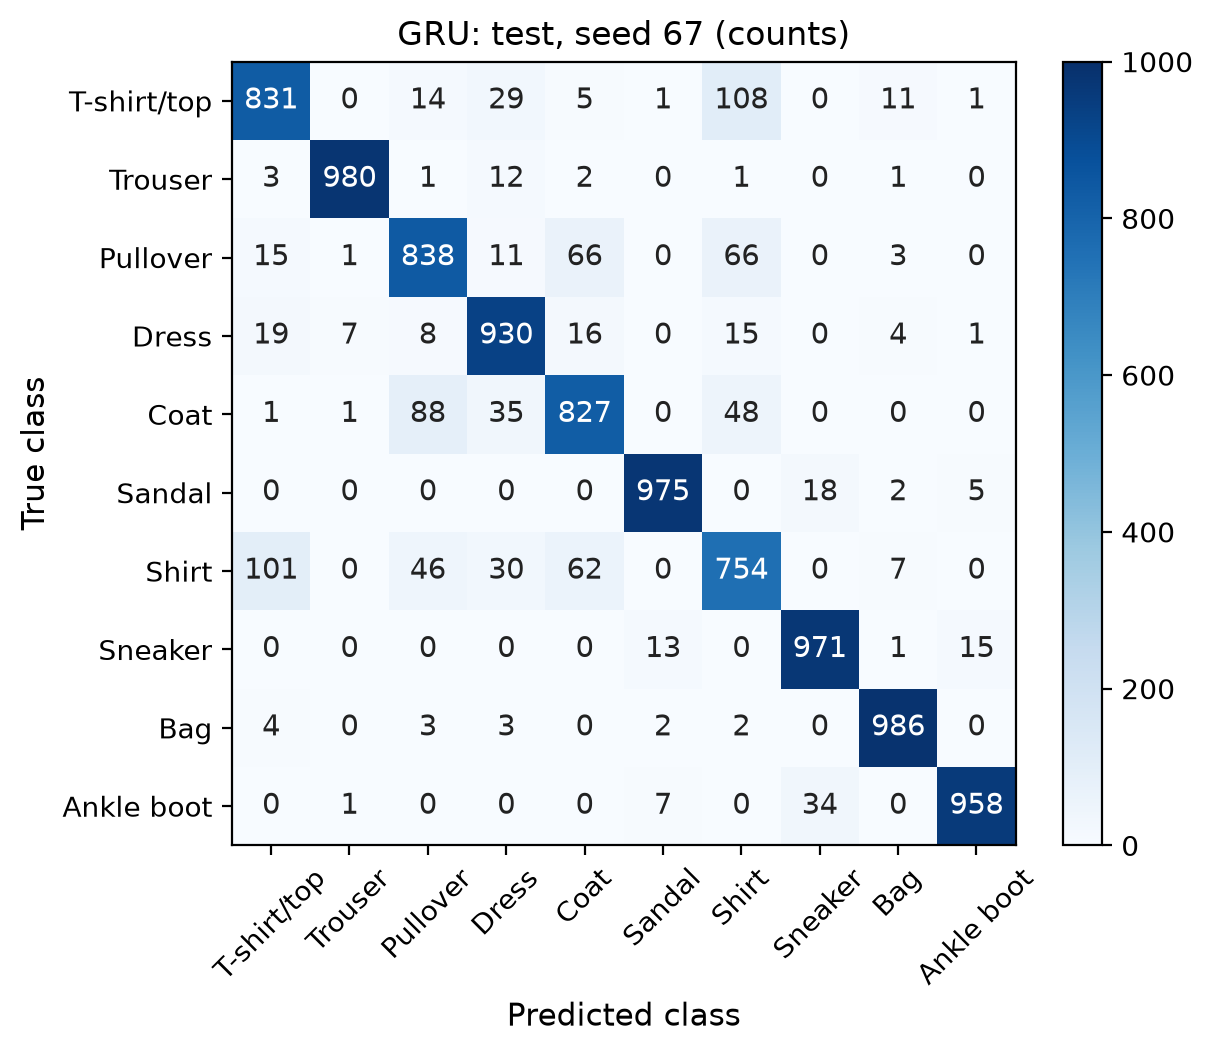
\includegraphics[width=.90\linewidth]{figures/confusion_rnn.png}
\caption{GRU test confusion counts, seed 67; shared color scale 0--1,000.}
\label{fig:cm-rnn}
\end{figure}
GRU reaches 90.50\% accuracy. Bag has its highest recall, 0.986; Dress
recall is 0.930. GRU has the highest Shirt recall among these five seed-67
models (0.754), although Shirt is still its lowest-F1 class (0.756).
Its overall score therefore does not reveal every class-level advantage.

\clearpage
\subsubsection{Transformer}
\begin{figure}[H]\centering
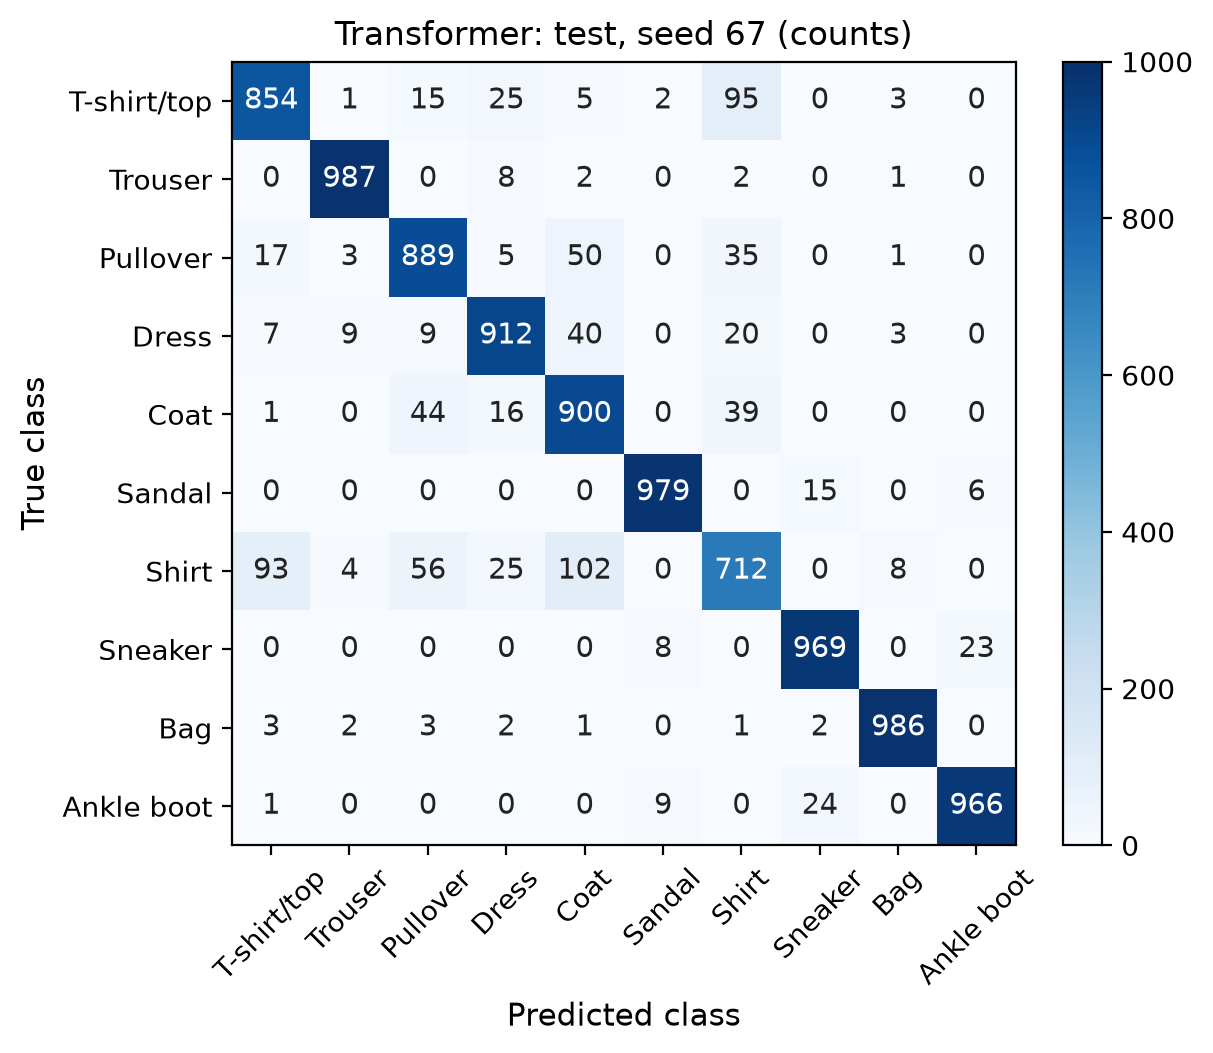
\includegraphics[width=.90\linewidth]{figures/confusion_transformer.png}
\caption{Transformer test confusion counts, seed 67; shared color scale 0--1,000.}
\label{fig:cm-transformer}
\end{figure}
Transformer reaches 91.54\% accuracy in seed 67 and has strong Bag
and Trouser F1 (0.985 and 0.984). Shirt remains weakest (F1 0.748), with 102
Shirts predicted as Coat, 93 as T-shirt/top and 56 as Pullover. Shirt precision
is higher than GRU's while recall is lower (0.712), illustrating a class-level
trade-off despite the strongest aggregate score.

\clearpage
\subsection{Qualitative Predictions and Error Analysis}
\label{sec:qualitative}
Each gallery below contains three correct, three difficult-correct and three
confidently incorrect examples from the same seed-67 test run. Correct examples
use the common IDs 0, 1 and 10 for all models; difficult-correct examples are
the three lowest-confidence correct predictions per model, and errors are the
three highest-confidence mistakes. Other IDs therefore vary across models.
The IDs identify official-test images; probabilities are rounded to three decimals.
These selected galleries illustrate behavior, not the prevalence of an error type.


\begin{figure}[H]\centering
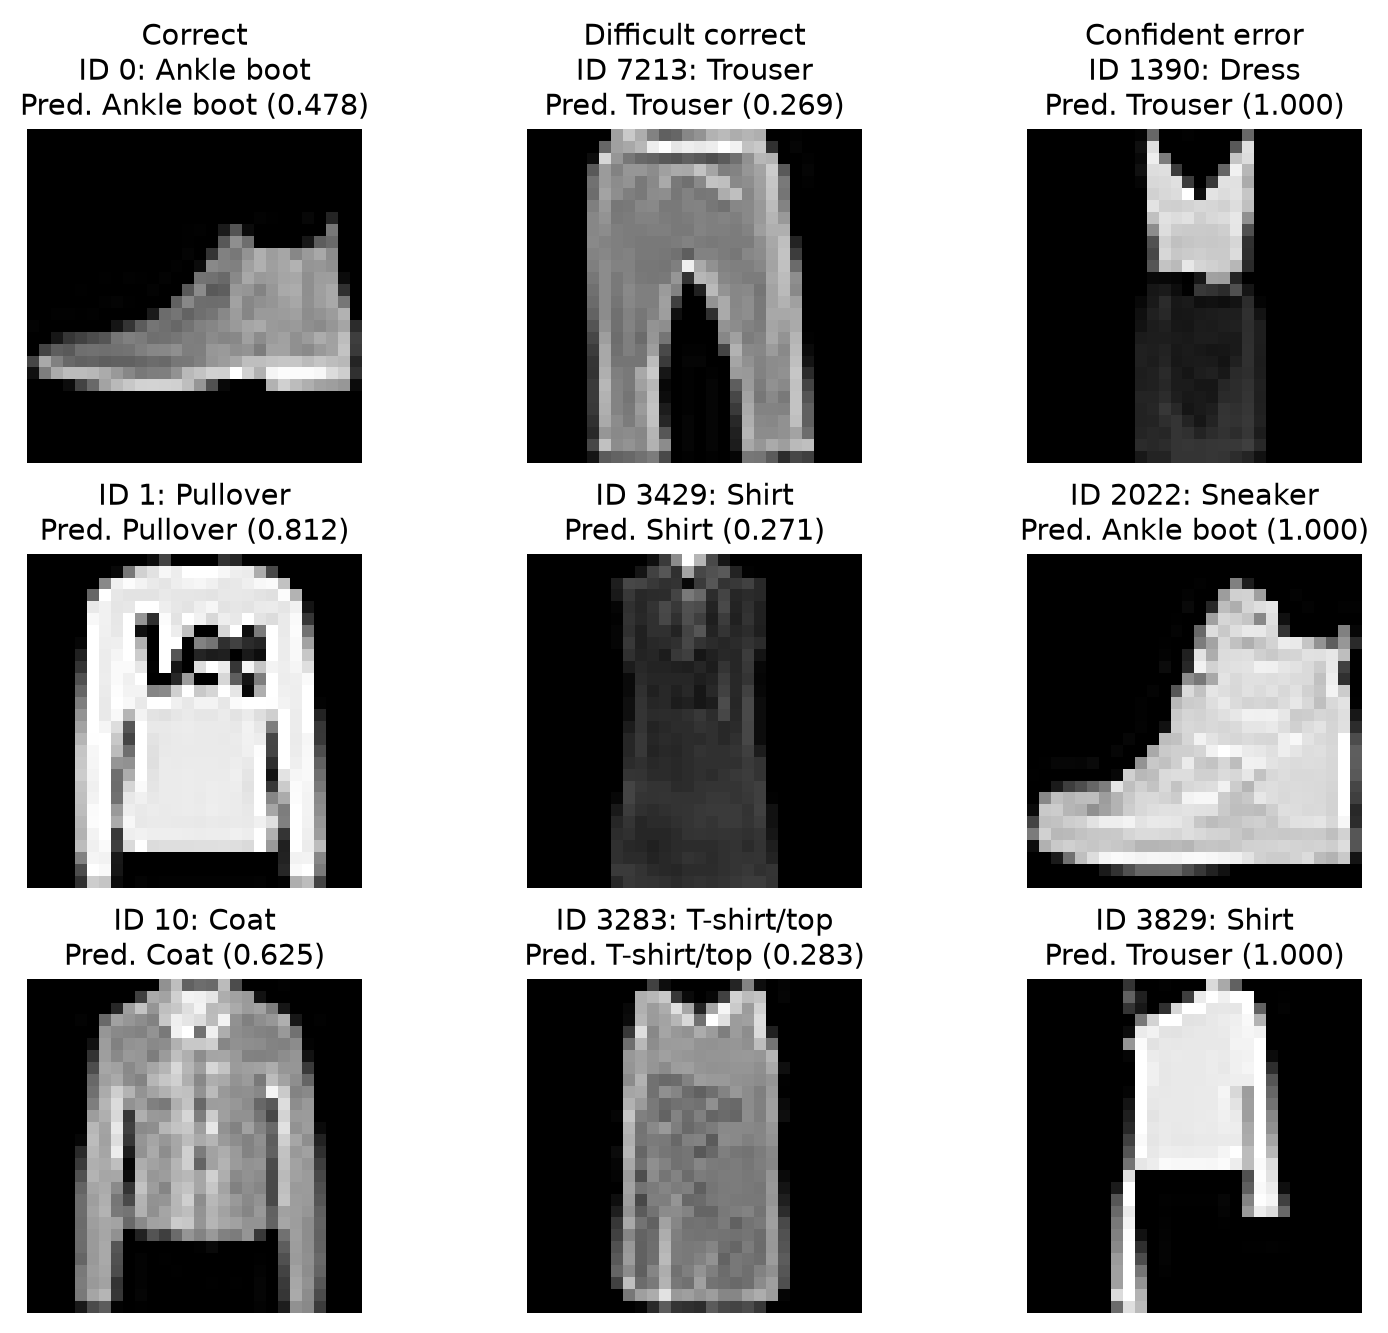
\includegraphics[width=.84\linewidth]{figures/gallery_linear.png}
\caption{Linear: common correct examples (left), low-confidence correct cases
(middle) and high-confidence errors (right), test seed 67.}
\label{fig:gallery-linear}
\end{figure}

\clearpage
\begin{figure}[H]\centering
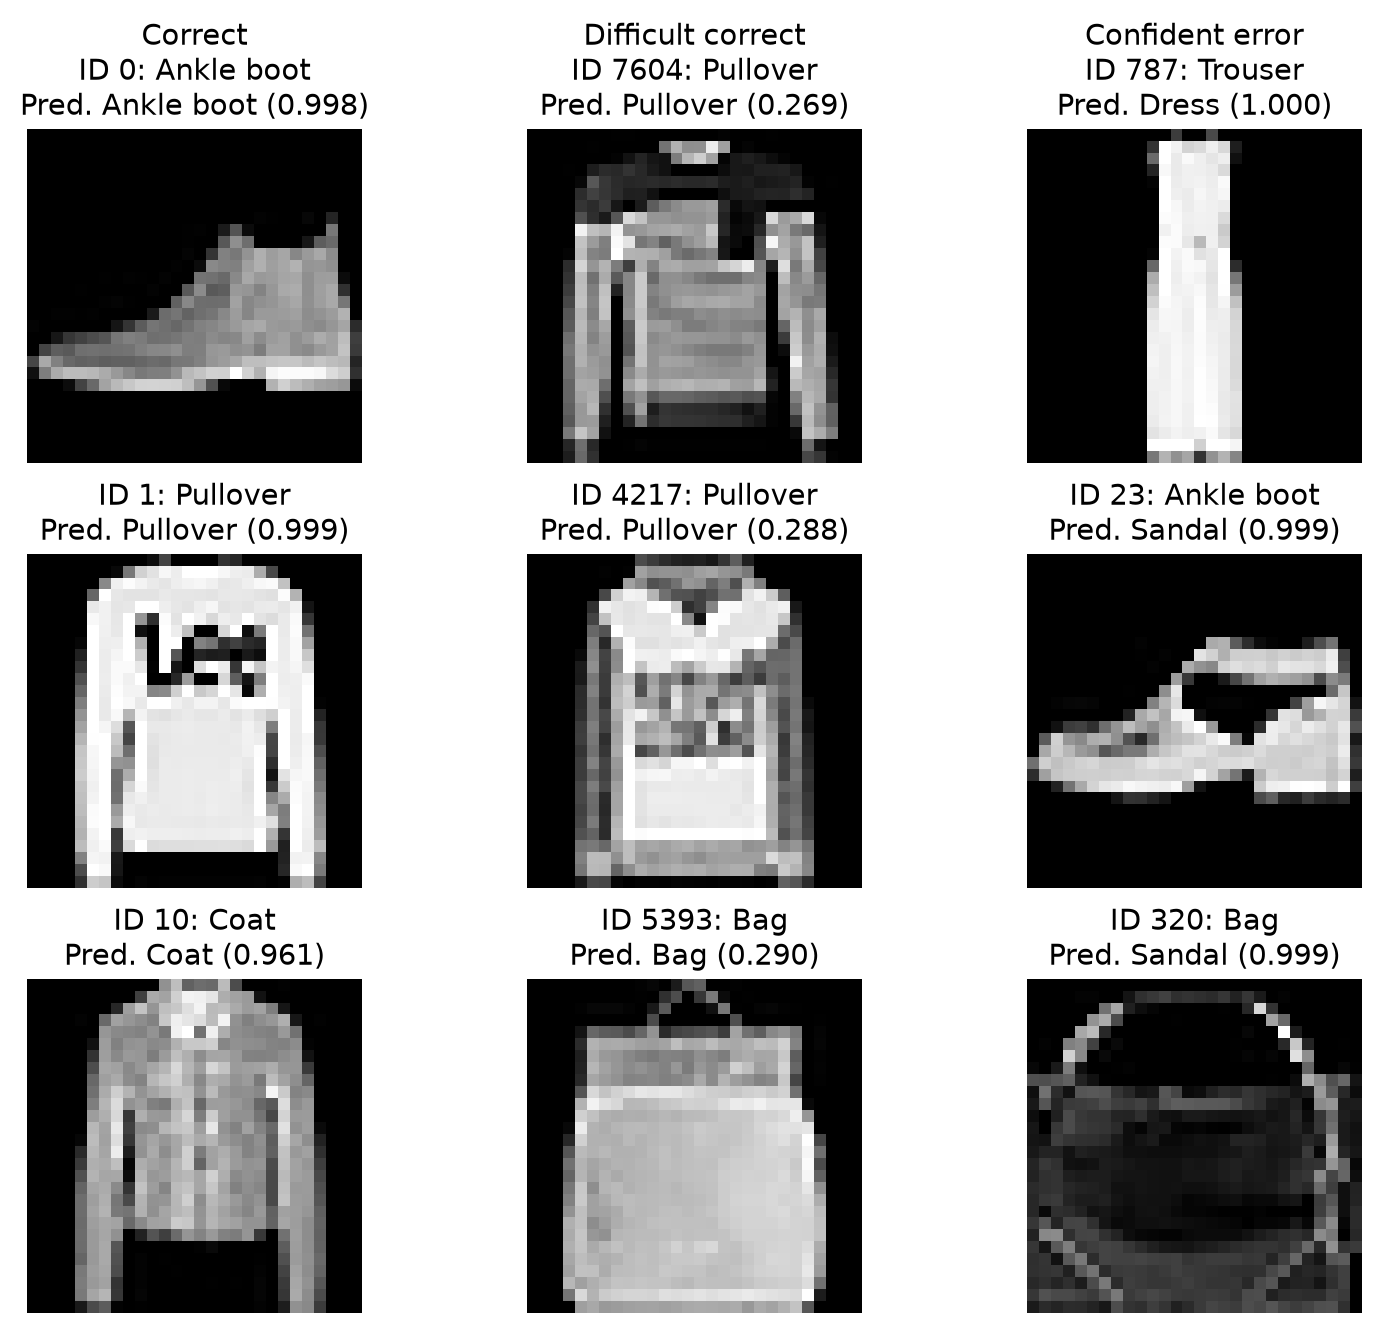
\includegraphics[width=.96\linewidth]{figures/gallery_mlp.png}
\caption{MLP: common correct examples (left), low-confidence correct cases
(middle) and high-confidence errors (right), test seed 67.}
\label{fig:gallery-mlp}
\end{figure}

\clearpage
\begin{figure}[H]\centering
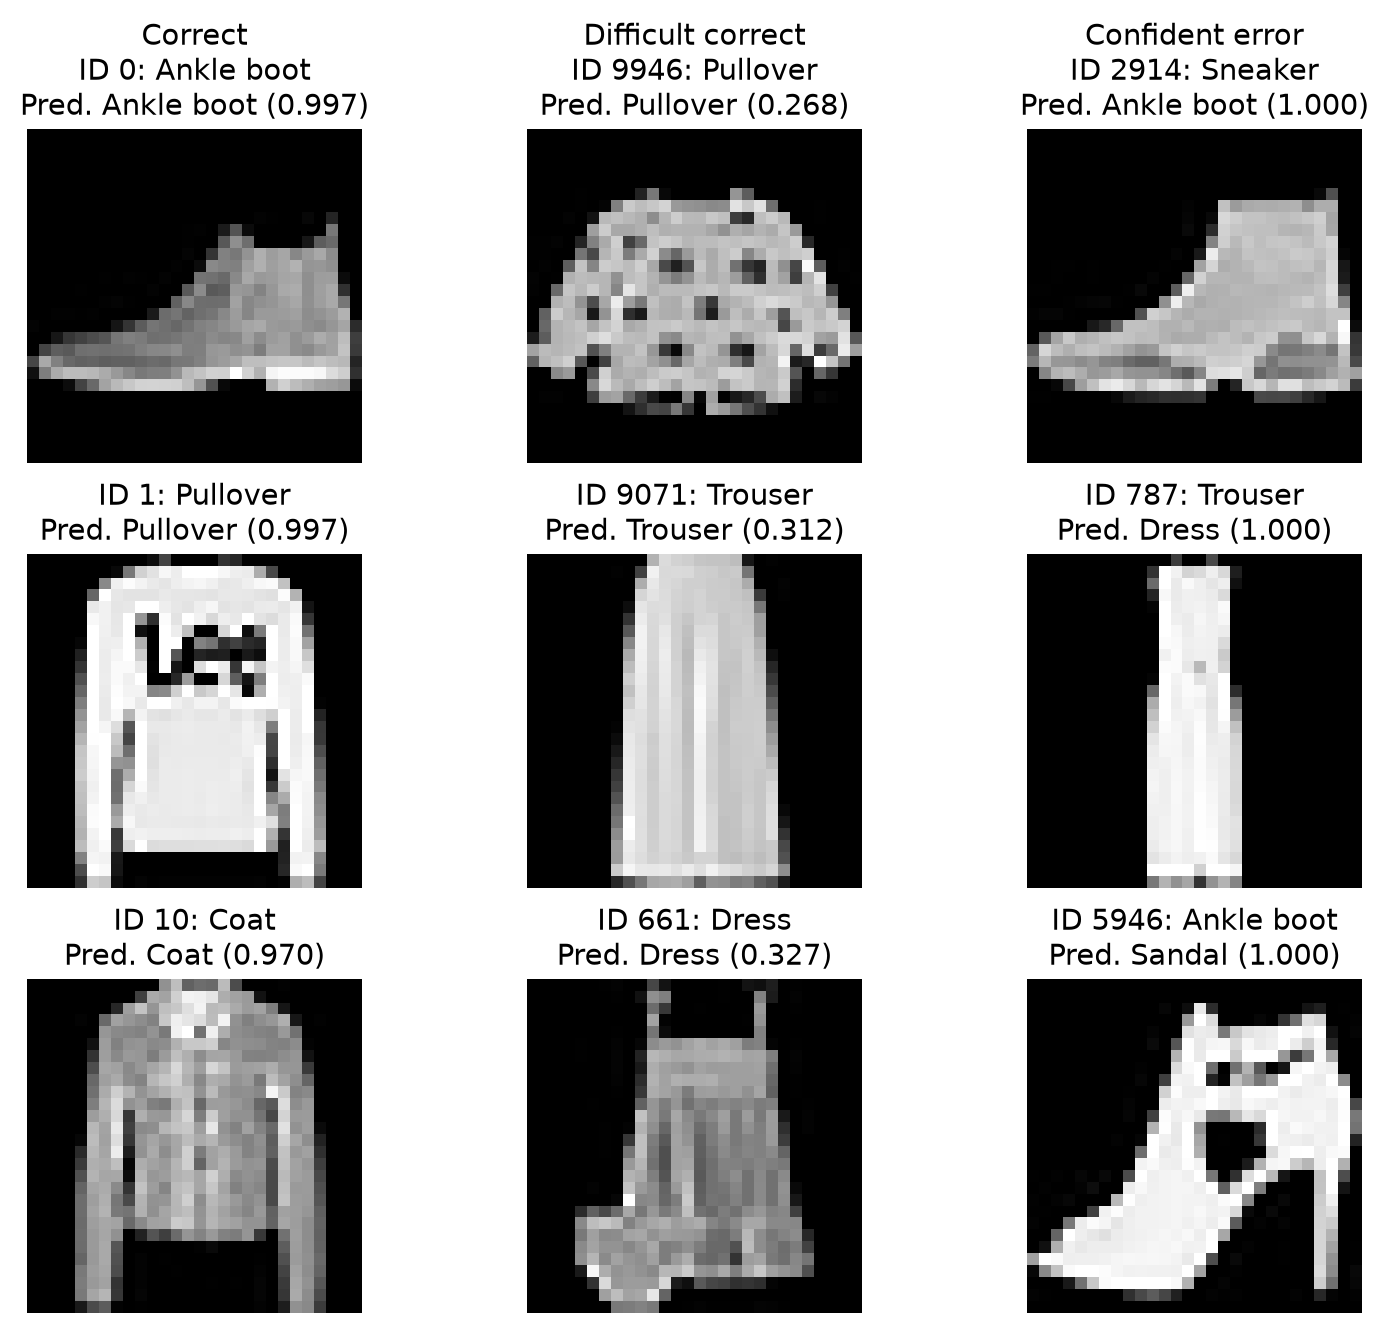
\includegraphics[width=.96\linewidth]{figures/gallery_cnn.png}
\caption{CNN: common correct examples (left), low-confidence correct cases
(middle) and high-confidence errors (right), test seed 67.}
\label{fig:gallery-cnn}
\end{figure}

\clearpage
\begin{figure}[H]\centering
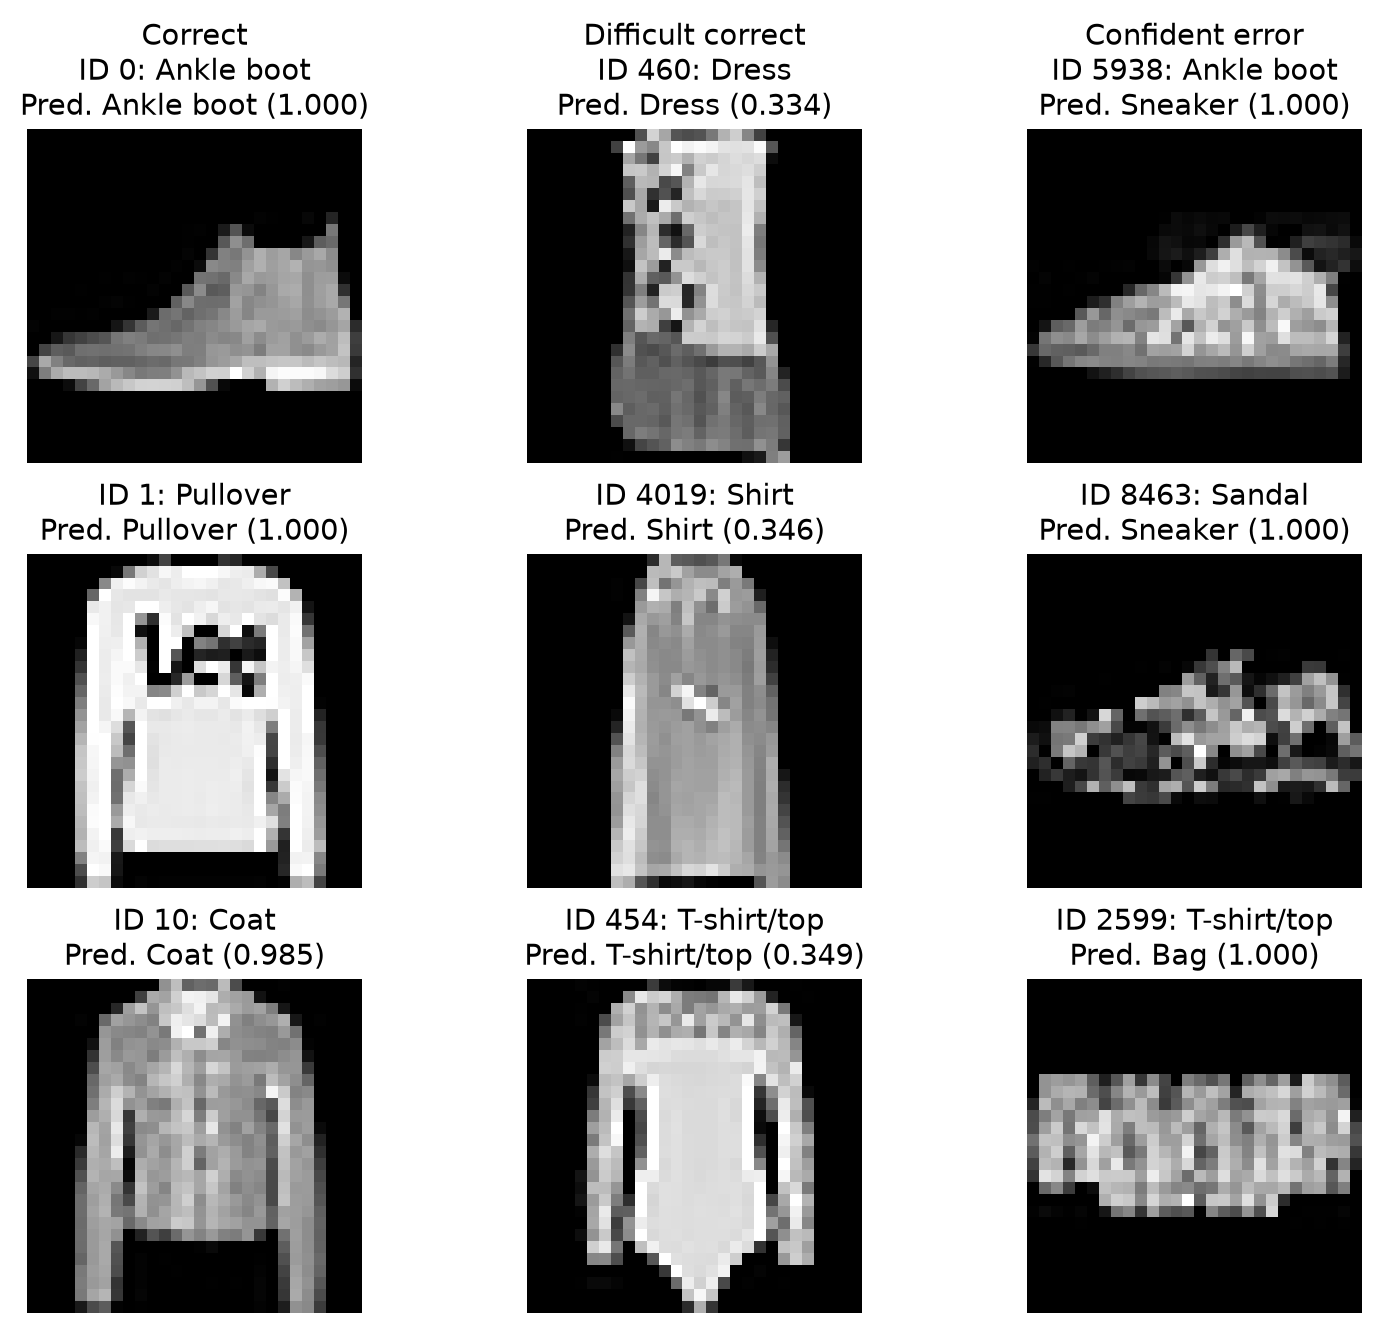
\includegraphics[width=.96\linewidth]{figures/gallery_rnn.png}
\caption{GRU: common correct examples (left), low-confidence correct cases
(middle) and high-confidence errors (right), test seed 67.}
\label{fig:gallery-rnn}
\end{figure}

\clearpage
\begin{figure}[H]\centering
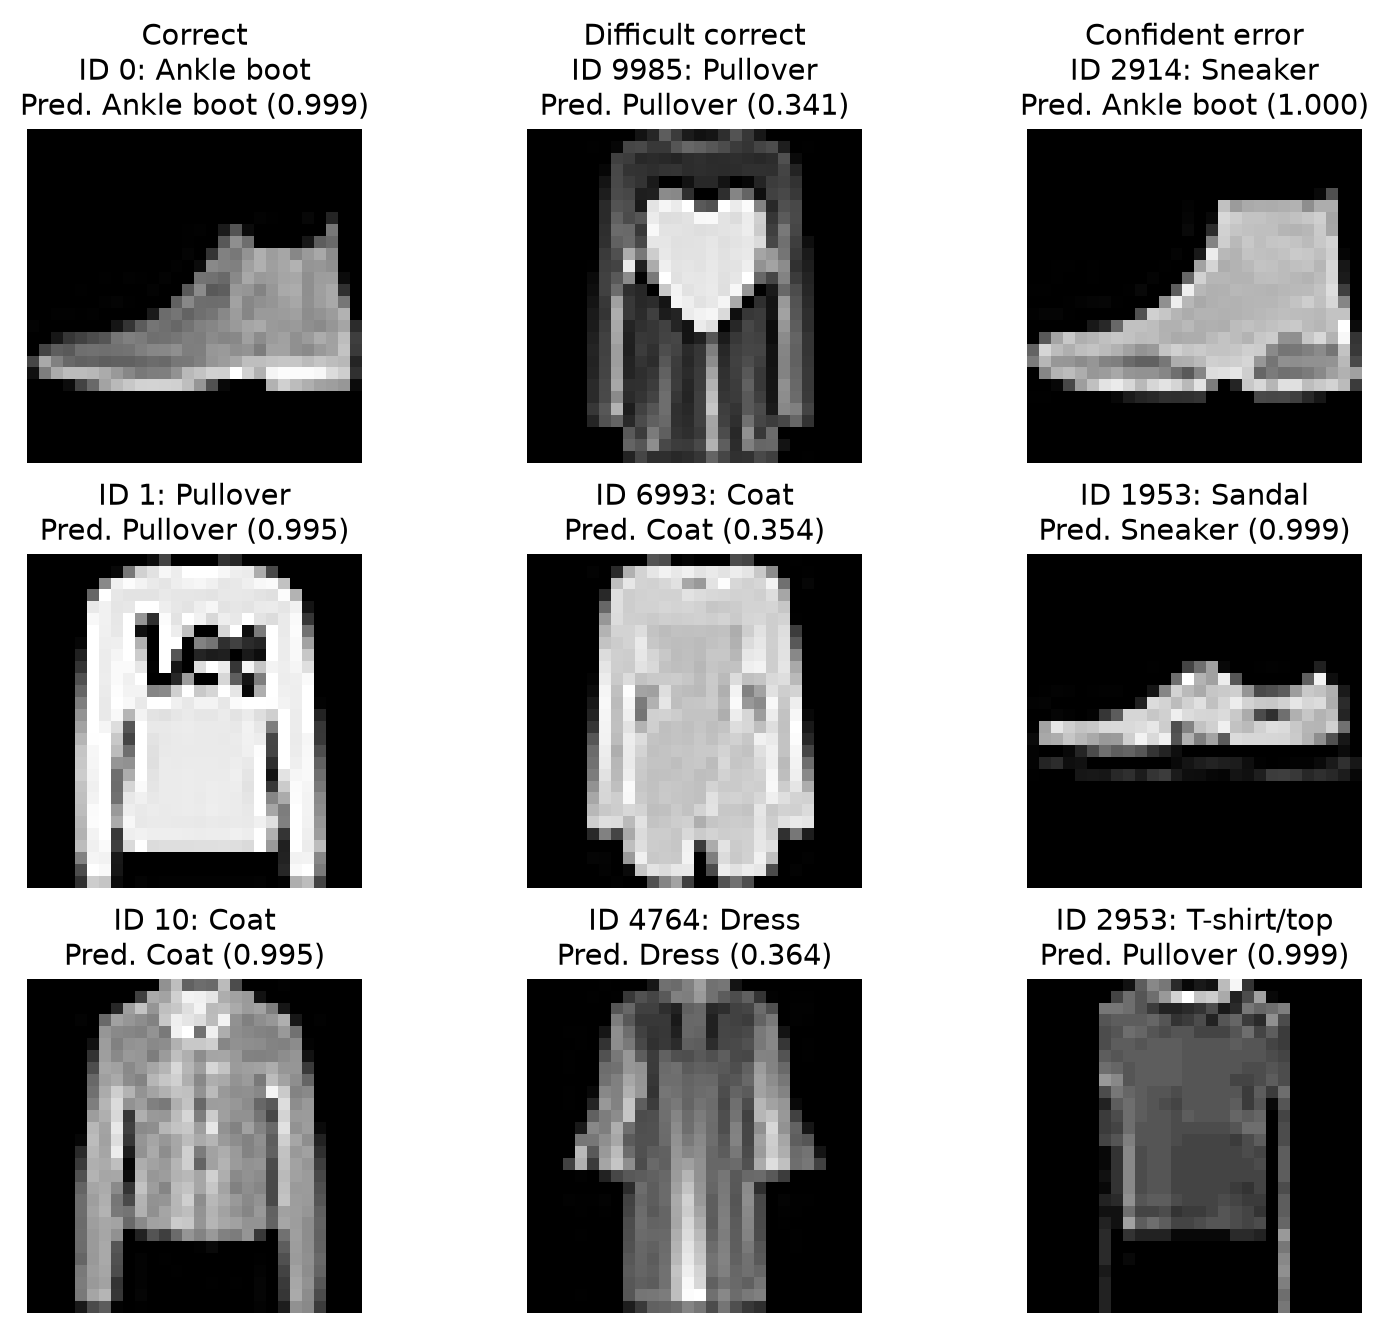
\includegraphics[width=.96\linewidth]{figures/gallery_transformer.png}
\caption{Transformer: common correct examples (left), low-confidence correct cases
(middle) and high-confidence errors (right), test seed 67.}
\label{fig:gallery-transformer}
\end{figure}

\FloatBarrier
The common example ID 0 (Ankle boot) is correct with confidence approximately
0.478 for Linear and near 1.0 for the nonlinear models. Conversely, both MLP
and CNN confidently predict Dress for true Trouser ID 787. Thus, a high softmax
score does not guarantee correctness. Low-confidence correct cases also show
that uncertainty and the final argmax label are distinct.

The class matrices quantify recurrent upper-body confusions; footwear galleries
show additional Sandal/Sneaker/Ankle-boot ambiguity. Plausible explanations are
shared silhouettes, limited resolution and missing texture cues, but the
present artifacts do not prove label errors or identify a unique cause.
Several focused follow-ups would address these patterns:
\begin{itemize}
\item Apparel confusions: inspect validated examples of Shirt/T-shirt/top/Coat/
Pullover and compare representations under matched training/parameter budgets.
This would test whether local or sequence features explain the observed gap.
\item Footwear confusions: measure pair-specific error rates and test a controlled
augmentation change while keeping model initialization and evaluation fixed.
The present galleries alone cannot establish whether augmentation would help.
\item Confident mistakes: assess reliability or calibration error on validation,
then evaluate a validation-fitted procedure under a fresh or preregistered
held-out protocol. A gallery is insufficient to claim population calibration.
\end{itemize}
These are proposed investigations, not completed ablations or promised gains.

\subsection{Representation and Inductive-Bias Discussion}
Linear assigns each class one global weighted pixel combination, with no hidden
feature hierarchy. Its low scores and severe apparel confusions are consistent
with limited expressiveness. Adding nonlinear dense layers improves test accuracy
by about 11.34 percentage points, but MLP remains below CNN and Transformer
despite having the largest parameter count.

The CNN's local connectivity and shared filters suit spatial image patterns.
It achieves close-to-leading quality with only 28,426 parameters. GRU instead
aggregates an ordered row sequence; its high seed-67 Shirt recall shows that
some class-level strengths are not captured by the overall ranking. No row/
column comparison was run, so the contribution of traversal order is unisolated.

The Transformer can combine information from distant patches through attention,
using learned position parameters to distinguish their locations. Its best
aggregate quality does not remove the shared Shirt/Coat ambiguity.
The results support these configurations as practical alternatives, but do not
prove that attention, locality or recurrence alone caused the measured differences.

\subsection{Limitations}
The evidence covers Fashion-MNIST, one effective configuration per family,
three seeds and one shared split. There is no matched-budget ablation, external
dataset, robustness benchmark or significance test. The repeated evaluations
reuse the same images, and selecting checkpoints on validation makes validation
scores optimistic for final comparison.

Epoch-loop cost combines training/validation and differs in completed epochs.
Training, classification evaluation and inference timing use distinct environments.
The Windows timing profile uses preallocated zeros and excludes I/O/transfer;
its amortized batch-64 cost does not predict batch-one or real-service latency.
Python patch-version variation, library differences and unrecorded friendly CPU
model name further limit exact cross-machine reproduction. The raw Windows timing
samples are retained; no unverified Colab timing table is substituted for them.

Example selection is deterministic but selective; images are not an uncertainty
or calibration sample. No perceptual-duplicate removal or independent label audit
was performed. The proposed explanations and follow-ups remain hypotheses.

\subsection{Conclusion}
The four research questions can be answered within these limits:
\begin{enumerate}
\item \textbf{Predictive quality.} Transformer leads at 91.267\% test accuracy
and 91.234\% macro-F1; CNN follows at 90.690\% and 90.726\%.
\item \textbf{Representation and errors.} Spatial and patch-token configurations
perform strongly, but similar apparel remains difficult. Architecture alone
was not isolated as the cause.
\item \textbf{Efficiency.} CNN has 72.9\% fewer parameters and 4.90 fewer
minutes of T4 epoch-loop time than Transformer. Their Windows CPU times are
0.404/0.445 ms per image; the preferred trade-off depends on the device.
\item \textbf{Seed consistency.} Test-accuracy SD is at most 0.324 percentage
points. All three paired Transformer--CNN differences are positive, without
establishing statistical significance.
\end{enumerate}
The measured outcome is a configuration-specific trade-off on Fashion-MNIST,
not a general ordering of architecture families for image classification.
\FloatBarrier
